\section{Scaling of Control Plane Service Chain}
\label{System-Design}
We first present the detailed design of \textit{ScalIMS} in deployment and scaling of the control plane (CP) service chain. %We start by discussing the scaling strategy used by CP service chain. The proactive scaling is governed by a proactive scaling protocol, whereas the reactive scaling is controlled by overload detection through runtime statistics. The proactive and reactive scaling of CP service chain are generic enough such that the DP service chain uses a similar scaling strategy with CP service chain with only minor difference. This section then presents how SIP messages are transmitted and manipulated on the CP service chain, so that data plane media flows could be routed over correct paths.

\subsection{Deployment and Entry Datacenter Binding}

%\subsubsection{Fixed CP Service Chain Placement}
The CP service chain consists of P-CSCF and S-CSCF. We use a fixed placement strategy by deploying P-CSCF instances on every datacenter and S-CSCF instances on a fixed selected datacenter, such that the delay between the datacenter where we place S-CSCF instances and other datacenters falls within an acceptable range (the acceptable SIP transaction completion time is typically 250ms).

%cut for space
%old
%The rationale behind such a fixed placement strategy is the following. S-CSCF instances constantly query the HSS database for user information, and they are usually built as a stateless network function by storing user location information (a temporary mapping between user name and user registration IP address) in a memcached cluster \cite{project-clearwater}. The stateless design improves load balancing among S-CSCF instances, but also implies that even if we spread S-CSCF instances over different datacenters, each S-CSCF instance still needs to access a central HSS server and a memcached cluster to process most of the SIP transactions. This fact urges us to place S-CSCF instances together with the HSS server and memcached cluster in the same selected datacenter. Since P-CSCF instances act as relay points for user flows to access S-CSCF instances, it is desirable to place P-CSCF instances on every datacenter, to facilitate user's access to a P-CSCF instance on the closest datacenter. This fixed placement strategy also simplifies the routing of SIP messages along the CP service chain. % and decisions on the number of CP VNF instances to be deployed in each datacenter.
%new
The rationale behind such a fixed placement strategy is the following. Even if we spread S-CSCF instances over different datacenters, each S-CSCF instance still needs to access a central HSS server and a memcached cluster to process most of the SIP transactions. This fact urges us to place S-CSCF instances together with the HSS server and memcached cluster in the same selected datacenter. Since P-CSCF instances act as relay points for user flows to access S-CSCF instances, it is desirable to place P-CSCF instances on every datacenter, to facilitate users' access to a P-CSCF instance on the closest datacenter. This fixed placement strategy also simplifies the routing of SIP messages along the CP service chain. % and decisions on the number of CP VNF instances to be deployed in each datacenter.

%\subsubsection{Entry Datacenter Binding}

\textit{ScalIMS} binds each user to the nearest datacenter according to his current geographical location, which is referred to as the user's {\em entry datacenter}. A user's CP and DP traffic can only enter and depart from the respective service chains from his entry datacenter. Such a datacenter binding is a natural design choice as each user should be pinned to a unique P-CSCF instance on a specific datacenter when he uses the IMS \cite{3gpp-ims}. %Choosing the geographically nearest datacenter decreases the possibility that the user experiences a large end-to-end delay between him and the entry datacenter.

To implement entry datacenter binding, a DNS server is maintained in \textit{ScalIMS}. When a user queries the IP address of an available P-CSCF instance by sending out a DNS request, the DNS server maps the user's IP address contained in the DNS request to a geographical location by querying an IP-location database ({\em e.g.}, IP location finder~\cite{iplocation}), referred to as the {\em location service}, and then assigns a datacenter that is closest to the user's current location as his entry datacenter.

%\subsubsection{Entry-exit Datacenter Pair}

When a call is initiated between user $a$ and user $b$, user $b$'s entry datacenter is also referred to as user $a$'s {\em exit datacenter}. In \textit{ScalIMS}, each pair of datacenters may form an entry-exit datacenter pair. CP workload and DP workload between each entry-exit datacenter pair are maintained in \textit{ScalIMS}, which are the aggregate rates of traffic that callers associated with an entry datacenter send to callees bound to the exit datacenter, along the CP service chain and the DP service chain, respectively. The traffic rates among entry-exit datacenter pairs are used for traffic prediction and VNF instance provision.

\subsection{Proactive Scaling}
\label{sec:CP_proactivescale}

\begin{figure}[h]
        \centering
        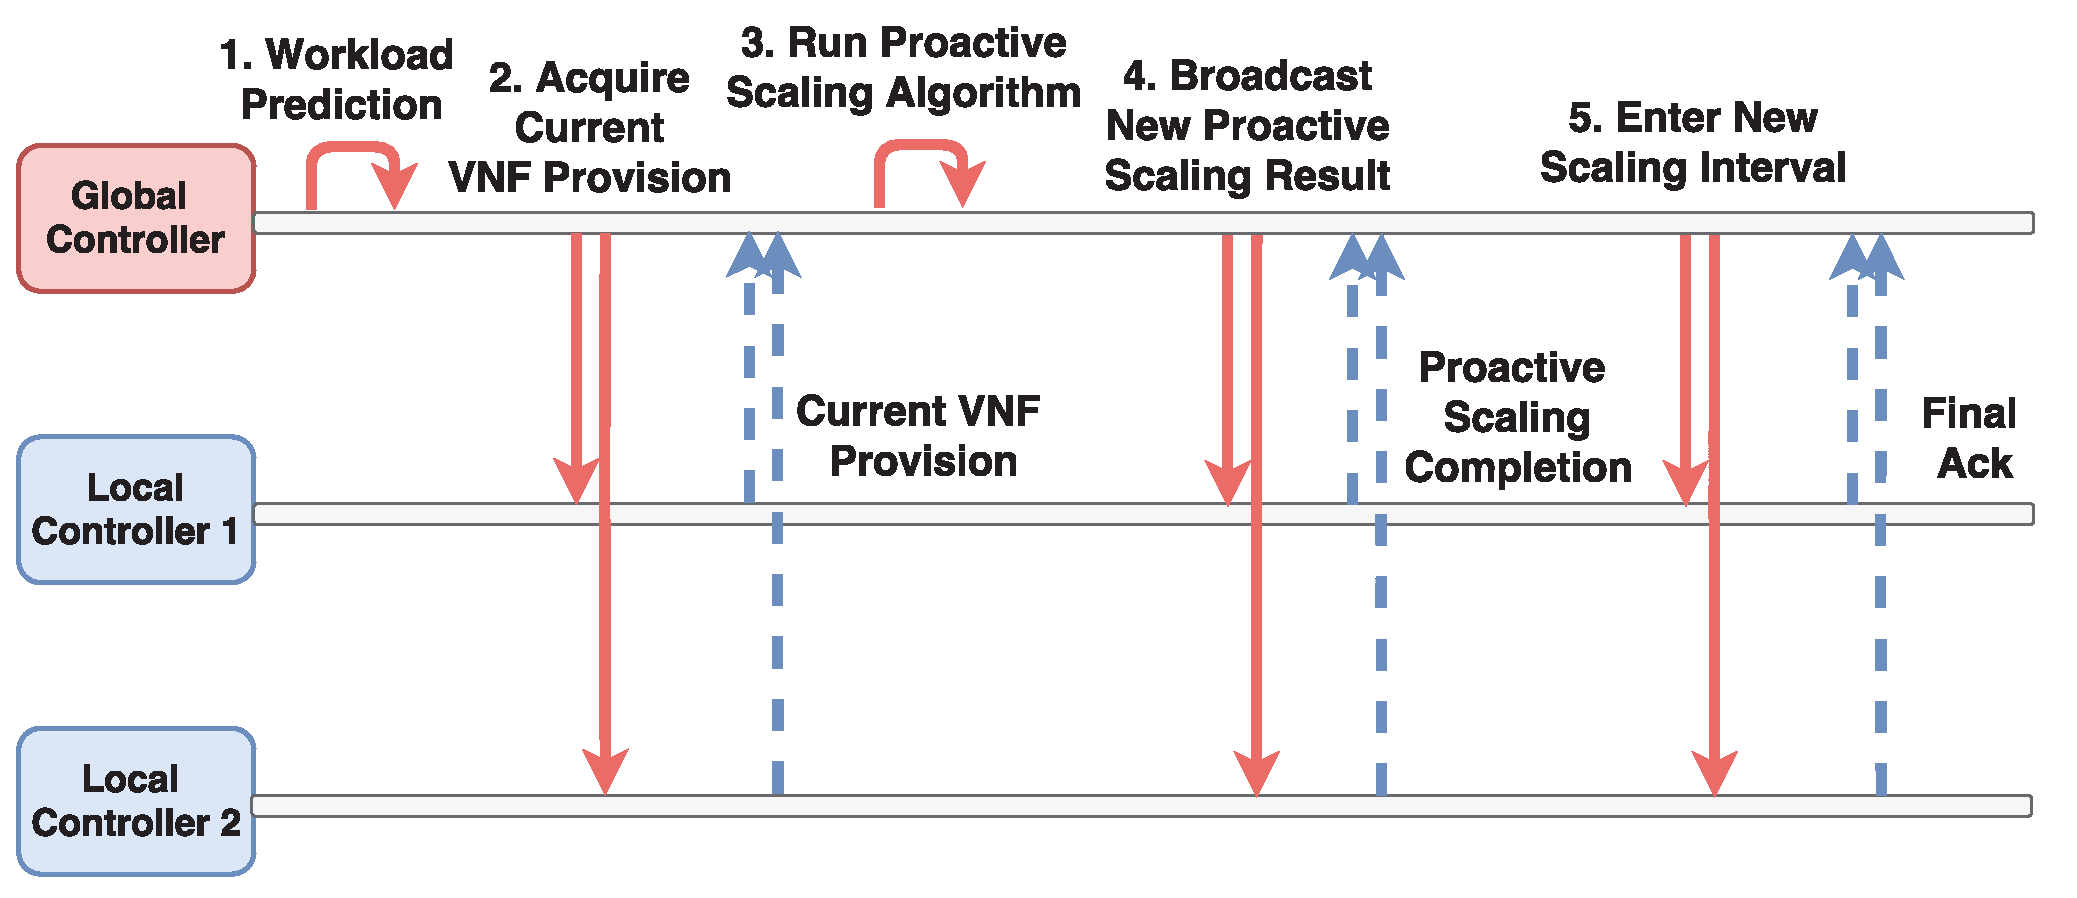
\includegraphics[width=1\columnwidth]{chap-scalims/figure/scaling-work-flow.eps}
        \caption{Proactive scaling protocol.}
        \label{fig:proactive-scaling}
\end{figure}

%cut for space
%old
%Proactive scaling is executed in each scaling interval according to the protocol illustrated in Fig.~\ref{fig:proactive-scaling}. The global controller and each local controller work in a request-response manner. In view of possible message loss, the global controller sets a re-transmision timer that re-transmits a request after 500ms, if no response is received.
%new
Proactive scaling is executed in each scaling interval according to the protocol illustrated in Fig.~\ref{fig:proactive-scaling}.

\noindent\textbf{1. Workload Prediction.}
Workload along a CP service chain is described by the number of SIP transactions carried out between each entry-exit datacenter pair every second. When a SIP transaction finishes, the S-CSCF instance involved uses the location service to determine which entry-exit pair this transaction belongs to (according to the IP addresses of the caller and the callee). Each S-CSCF instance keeps a record of the number of SIP transactions on each entry-exit datacenter pair and reports this number to the local controller in its datacenter every second. The local controller accumulates CP workload for 5 seconds before relaying it to global controller.

At the end of a scaling interval $t$, the global controller predicts the workload $\hat{u}_{t+1}$ in the next scaling interval using historic data in past several intervals (10 as in our experiments), using auto regression~\cite{wood2007black}: $\hat{u}_{t+1} = \mu + \phi(u_t-\mu)$.
%\begin{equation}
%\hat{u}_{t+1} = \mu + \phi(u_t-\mu)
%\end{equation}
%\noindent
Here $\mu$ is the mean of the historic workload values in the past several scaling intervals, $u_t$ is the average CP workload collected in the current interval, and $\phi$ can be decided using the covariance of the historical workload divided by the variance of the historical workload. The workload between each entry-exit datacenter pair is predicted this way.

\noindent\textbf{2. Acquire Current VNF Provision.} The global controller then broadcasts a message to local controllers, asking them to send %information of the current VNF instance provisioning,
 the numbers of instances of each VNF provisioned in the respective datacenter. Upon receiving this request, a local controller knows that proactive scaling computation is on going, stops its reactive scaling process (Sec.~\ref{sec:CP_reactivescale}) so that it does not interfere with proactive scaling, and then sends its current VNF provision information to the global controller.

\noindent\textbf{3. Run Proactive Scaling Alrogihm.} After receiving current VNF deployment from all local controllers, the global controller computes the numbers of P-CSCF and S-CSCF instances to be deployed in each datacenter in the next scaling interval. Since all S-CSCF instances are placed in the same datacenter, the number is decided by dividing the total predicted workload between all pairs of entry-exit datacenters by the processing capacity of S-CSCF. The number of P-CSCF instances to be deployed in a datacenter is computed by dividing the overall predicted workload for the entry-exit datacenter pairs, which use this datacenter as either entry or exit datacenter, by the processing capacity of P-CSCF.

\noindent\textbf{4. Broadcast Proactive Scaling Result.} The global controller then broadcasts the computed numbers to local controllers. A local controller sends a completion message to the global controller, after creating new VNF instances (scale-out) or enqueueing unused VNF instances to the respective buffer queues (scale-in), according to the received numbers.

\noindent\textbf{5. Enter New Scaling Interval.} After the global controller receives completion messages from all local controllers, it broadcasts an ``enter new scaling interval'' message to all local controllers. After receiving this message, a local controller increments its scaling interval index by 1, and shuts down some VNF instances from the head of the buffer queues. Then the local controller sends a final acknowledgement to the global controller. Upon receiving all final acknowledgements, % from all local controllers,
 the global controller increases its scaling interval index by 1.

\textit{Buffer Queue.} In each datacenter, a double-ended buffer queue is maintained to temporarily hold unused VNF instances, with one queue for one type of VNF. When a VNF instance is to be removed, instead of directly shutting it down, the local controller tags it with the index of the current scaling interval, and enqueues it to the tail of the respective buffer queue. Once a VNF instance is enqueued, no more flows will be routed to it. Whenever more instances of a VNF are to be established, if there are available instances in the buffer queue of this VNF, buffered instances will be popped out from the tail of the queue, and transformed back to working instances, to fulfil the demand as much as possible. The purpose is to avoid creating new VNF instances frequently and improve flow loss rate, as the typical VNF creation time can last a few seconds and has a bad influence on flow loss rate. Unused buffered VNF instances are destroyed after $\tau$ scaling intervals ($\tau$ is set to 10 in our implementation), in Step 5 above.
%: when the local controller in the datacenter receives an ``enter new scaling interval message'', it checks from the head of each buffer queue whether an instance has been enqueued $\tau$ intervals ago; if so, the VNF instance at the head will be dequeued. Dequeuing repeats until all unused instances for $\tau$ intervals are cleaned. These dequeued VNF instances gets destroyed by local controller when there's no active traffic on them.
% The local controller will destroy dequeued VNF instances until there's no active traffic on them.

\vspace{-3mm}
\subsection{Reactive Scaling}
\label{sec:CP_reactivescale}

%Duan's new:
%address some problems
An agent running on each VNF instance reports to the local controller runtime statistics of the instance, e.g., CPU usage, memory usage and the number of input packets, in each second. The local controller maintains time series of these statistics for each VNF instance. It decides whether CPU, memory, or network is overloaded during the past several seconds by comparing the respective statistics with a threshold (Sec.~\ref{Evaluation}). If overload is persistently identified for at least two types of statistics ({\em e.g.}, CPU and network usage) for some consecutive time (5 seconds as in our experiments), then that VNF instance is reported as overloaded. We make the decision using two types of statistics in order to eliminate false alarms brought by examining a single statistics. The local controller then avoids routing new traffic flows ({\em i.e.}, new calls) to overloaded instances if there are other available instances. In a datacenter, if the states of a majority of instances of a VNF are ``overloaded'', scale-out is triggered by adding one new instance of that VNF. Note that no scale-in decisions (i.e., removing instances) are made reactively. They are solely handled by the proactive scaling protocol, as it improves system stability during workload fluctuation.
%Because efficient reactive-scale-in requires support of dynamic flow migration \cite{gember2014opennf} to quickly shutdown idle VNF instances, which is hard to implement.

\subsection{Flow Routing on Control Plane}
\label{sec:message-routing-on-control-plane}

When a user connects to the IMS system, he first issues a query to a DNS server, which determines the entry datacenter of this user and obtains the IP address of an available P-CSCF instance (non-overloaded) by querying the local controller of the entry datacenter. A P-CSCF instance learns the IP addresses of several available S-CSCF instances (non overloaded) by querying the local controller of the datacenter hosting S-CSCF instances and distributes its up-stream requests to these S-CSCF instances evenly. It regularly (every 30s in \textit{ScalIMS}) updates the connections to up-stream S-CSCF instances by querying the local controller to obtain an updated view of S-CSCF instances.


%explain how flows are routed in case of P-CSCF and S-CSCF scale-in and scale-out.


%we must state the SIP message manipulation here, as the routing of data plane flows will use these mappings to obtain flow's service chain path
A CP flow for establishment of a call (i.e., a SIP INVITE transaction) runs as follows.
The caller sends out a SIP INVITE message, carrying caller's source IP address, receive port and send port, to the assigned P-CSCF instance.
%A SIP INVITE message carries the caller's source IP address, receive port and send port.
The P-CSCF instance forwards the message to one connected S-CSCF instance.  The
S-CSCF instance queries the HSS database to obtain the P-CSCF instance assigned
to the callee that is saved when callee registers himself, and forwards the SIP
INVITE message to that P-CSCF instance. The P-CSCF instance assigned to the
callee modifies the source IP field in the message to an IP address located on
the callee's entry datacenter, so that the callee can learn an IP address
located on callee's entry datacenter. The P-CSCF instance then sends the
modified SIP INVITE message to the callee.  The callee responds with a SIP OK
message, going through the same service chain in the reversed direction. When
the SIP OK message passes through caller's entry datacenter, the P-CSCF instance
modifies source IP field in the message to an IP address located on caller's
entry datacenter as well. When such a SIP INVITE transaction ends, the
caller and the callee use the learned IP addresses as the destination IP addresses of the DP media flows and send their media flows to their entry datacenters, from where the media flows enter the DP service chain.

%The content of these two messages are modified by the P-CSCF instance in order for the caller/callee to learn a destination IP address on his entry datacenter.  When a SIP INVITE message passes through callee's entry datacenter, the source IP field is modified to an IP address located on the callee's entry datacenter, so that the callee learns about a destination IP address located on callee's entry datacenter. A similar process is applied to SIP OK message when the message passes through caller's entry datacenter as well.


Besides SIP message modification, a P-CSCF instance sends two mappings (Table~\ref{mappings}) to its local controller after it has received the SIP OK message. The local controller saves these mappings for use when processing the DP flows (Sec.~\ref{sec-dp-scaling}). %The saved mapping differs depending on whether the P-CSCF instance is on caller's or callee's entry datacenter.



\begin{table}[t]
	\caption{Mappings saved on local controller}% of entry datacenter}
	\label{mappings}
\centering
\resizebox{\columnwidth}{!}{%
\begin{tabular}{| l |p{0.75\columnwidth}|}
\hline
\multirow{2}{*}{\begin{tabular}[c]{@{}l@{}}Controller on\\ Caller Entry DC\end{tabular}} & 1. (caller IP, caller send port)$\rightarrow$(callee IP)                   \\ \cline{2-2}
                                                                                & 2. (callee IP, callee send port)$\rightarrow$(an IP on caller's entry datacenter, caller IP, caller receive port) \\ \hline
\multirow{2}{*}{\begin{tabular}[c]{@{}l@{}}Controller on \\ Callee Entry DC \end{tabular}} & 3. (callee IP, callee send port)$\rightarrow$(caller IP)                   \\ \cline{2-2}
                                                                                & 4. (caller IP, caller send port)$\rightarrow$(an IP on callee's entry datacenter, callee IP, callee receive port) \\ \hline
\end{tabular}
}
\end{table}
